\section{Worksheet 3}
To create a primitive object, like for example a plane, we have to provide:
\begin{itemize}
	\item  a path to an .mtl file which defines a list of materials and the related properties for each one of them
	\item an id which indicates which material the object is made between the ones defined in the .mtl file.
\end{itemize}
One of the properties defined in the .mtl file is also the path to a texture image.\\
To implement the texturing of the plane we have to calculate the relative texture coordinates.
\begin{lstlisting}
void Plane::get_uv(const float3& hit_pos, float& u, float& v) const 
{ 	
	u = dot(onb.m_tangent,(hit_pos-position))*tex_scale;
	
	v = dot(onb.m_binormal, (hit_pos - position))*tex_scale;
}

bool Plane::intersect(const Ray& r, HitInfo& hit, unsigned int prim_idx) const
{	
	float t1 = -(dot(r.origin, onb.m_normal) + d) / dot(r.direction, onb.m_normal);
	bool intersect = dot(r.direction, onb.m_normal) != 0;
	bool has_hit =  intersect && t1 > r.tmin && t1 < r.tmax;
	if (has_hit){
		hit.has_hit = true;
		hit.dist = t1;
		hit.position = r.origin + (r.direction * t1);
		hit.geometric_normal = normalize(onb.m_normal);
		hit.shading_normal = normalize(onb.m_normal);
		hit.material = &material;
		if (material.has_texture) {
			float u;
			float v;
			get_uv(hit.position, u, v);
			hit.texcoord=make_float3(u,v,0);
		}
	}
	return has_hit;
}
\end{lstlisting}
When we render an object if it doesn't have a texture we define it's emission as the ambient coefficient of the material of the object, otherwise we divide the ambient coefficient by the diffuse coefficient and we multiply it by the texture color.
\begin{figure}[H]
	\centering
	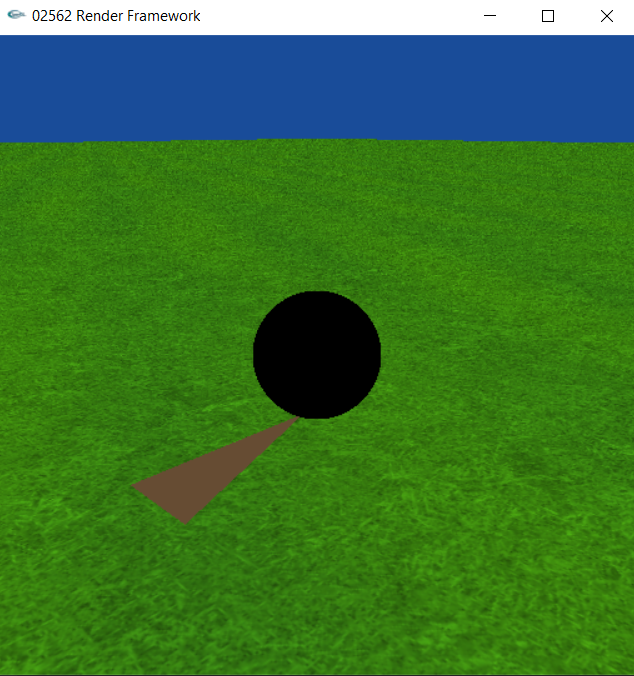
\includegraphics[scale=\imagescale]{images/worksheet_3/part_4}
	\caption{Grass texture on plane}
	\label{fig:texture_plane}
\end{figure}
In figure \ref{fig:lookup_comparison} we can examine a comparison between the results of nearest and linear look-up. As we can see in this example the results look almost identical.
\begin{figure}[H]
	\centering
	\subfloat[\centering Nearest lookup]{{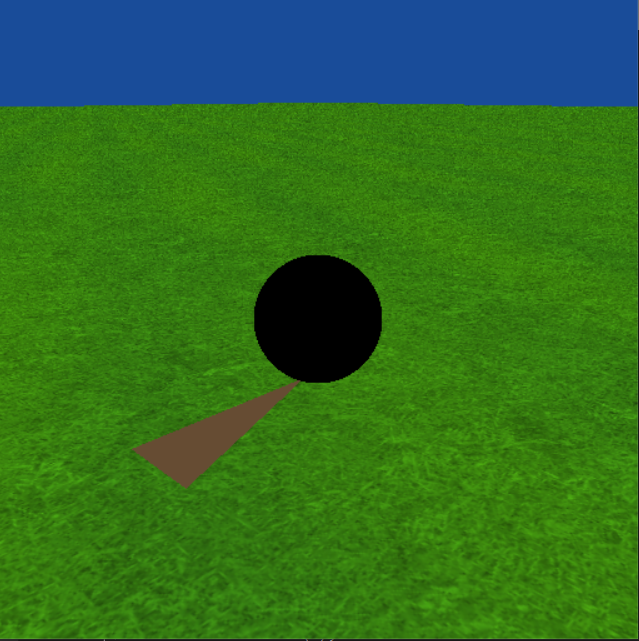
\includegraphics[width=5cm]{images/worksheet_3/nearest} }}%
	\qquad
	\subfloat[\centering Linear lookup]{{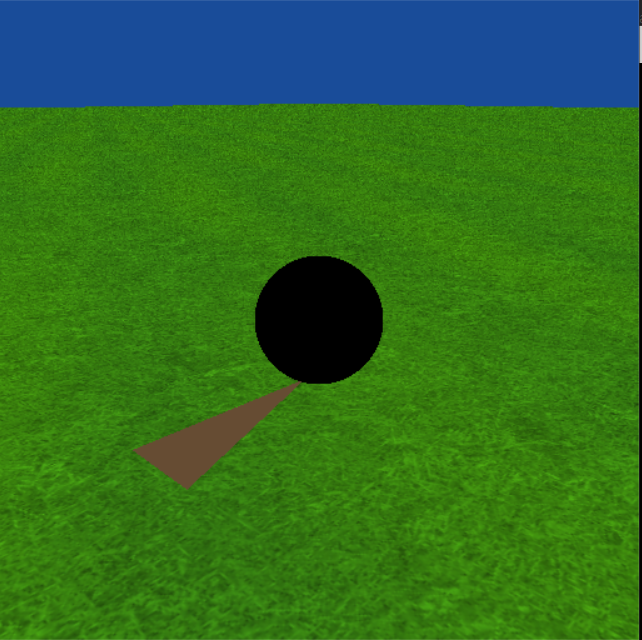
\includegraphics[width=5cm]{images/worksheet_3/linear} }}%
	\caption{Comparison between nearest and linear lookup}%
	\label{fig:lookup_comparison}%
\end{figure}
In figure \ref{fig:lookup_comparison} we can see how the tex\_scale parameter affects our results. With a really low texture scaling value the texture get's spreaded on the whole surface of the plane and it get's repeated much more rarely. On the other hand with a really high texture scaling value the texture appears much smaller on the surface of the plane and the same patterns get repeated much more often.
\begin{figure}[H]
	\centering
	\subfloat[\centering Low tex\_scale]{{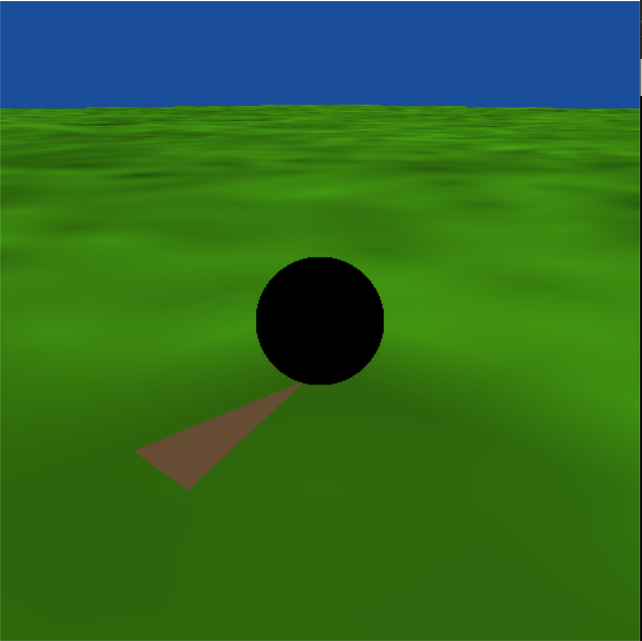
\includegraphics[width=5cm]{images/worksheet_3/low_tex_scale} }}%
	\qquad
	\subfloat[\centering High tex\_scale]{{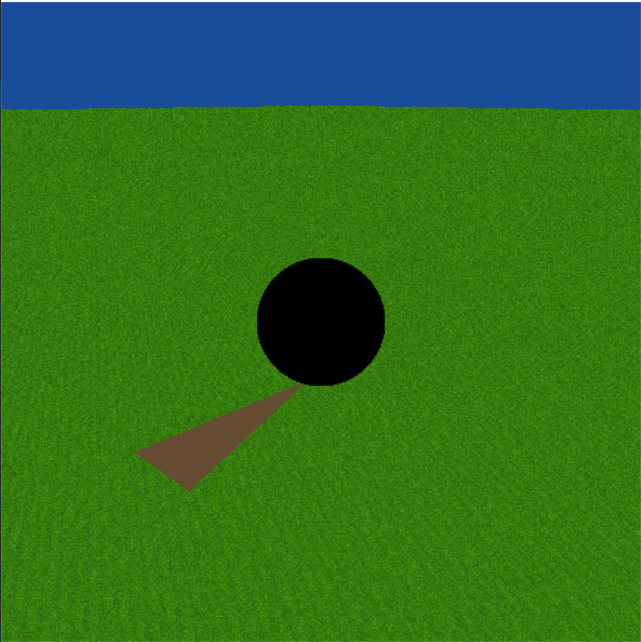
\includegraphics[width=5cm]{images/worksheet_3/tex_scale_10} }}%
	
	\caption{Comparison between High and Low tex\_scale}%
	\label{fig:tex_scale_comparison}%
\end{figure}
By implement an inverse sphere mapping we can calculate the uv-coordinates necessary to texture a sphere. The result can be seen in figure \ref{fig:textured_sphere} 
\begin{lstlisting}
void InvSphereMap::project_direction(const float3& d, float& u, float& v) const
{
	float3 ve = normalize(d);
	float teta = acos(ve.x);
	float fi = atan2(ve.y, ve.x);
	u = teta / M_PIf;
	v = fi / 2 * M_PIf;
}
\end{lstlisting}

\begin{figure}[H]
	\centering
	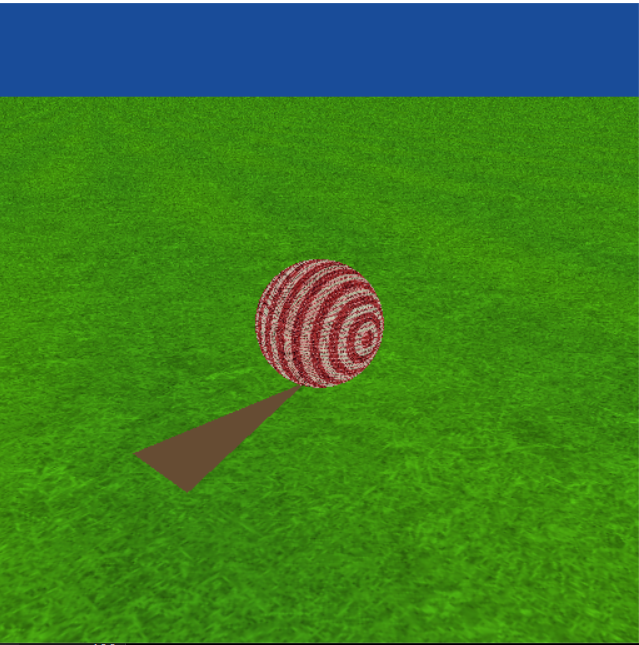
\includegraphics[scale=\imagescale]{images/worksheet_3/textured_sphere}
	\caption{Textured sphere}
	\label{fig:textured_sphere}
\end{figure}